%%%%%%%%%%%%%%%%%%%%%%%%%%%%%%%%%%%%%%%%%%%%%%%%%%%%%%%%%%%%%%%
% 音講論用スタイルファイル onkoron.sty の使用例
%
% 作成：2005年4月 9日 (初版)
%             4月15日 (Ver.1)
%             4月27日 (Ver.1.1)
%       2013年6月11日 (Ver.1.2)
%
%%%%%%%%%%%%%%%%%%%%%%%%%%%%%%%%%%%%%%%%%%%%%%%%%%%%%%%%%%%%%%%
\documentclass[10pt,twocolumn,dvipdfmx]{jarticle} % 11pt(標準)
%\documentclass[11pt,dvipdfmx]{jarticle} % 11pt(標準)
%\documentclass[10pt,twocolumn]{jarticle} % 10pt(オプション)
\usepackage{onkoron}
\usepackage{amsmath,amssymb,nccmath}    % 数式
\usepackage{bm}
\usepackage{graphicx} 
\usepackage{algpseudocode}
\usepackage{algorithm}
\usepackage{booktabs}

%%%%%%%%%%%%%%%%%%%%%%%%%%%%%%%%%%%%%%%%%%%%%%%%%%%%%%%%%%%%%%%
% 参考文献の引用が [3,6,2,1] -> [1-3,6] になります．
% citesort.sty は，2005年4月現在，下記からダウンロード可能です．
% http://www.utexas.edu/ogs/etd/LaTeX/Style.files/citesort.sty
%
%\usepackage{citesort}

%%%%%%%%%%%%%%%%%%%%%%%%%%%%%%%%%%%%%%%%%%%%%%%%%%%%%%%%%%%%%%%
% 行間を標準よりも広くしたい場合には，ここの数字を大きくして
% ください．逆に狭くしたい場合には，数字を小さくしてください．
\renewcommand{\baselinestretch}{1.0}

%%%%%%%%%%%%%%%%%%%%%%%%%%%%%%%%%%%%%%%%%%%%%%%%%%%%%%%%%%%%%%%
% 論文タイトルおよび脚注用の英文を記載する．

\title{
単チャネルCross-Relation法に基づく時間周波数領域ブラインド残響除去
%音源振動を補助情報とする時間領域単チャネル残響除去
\thanks{
  本研究は，科学技術振興機構（JST）創発的研究支援事業（JPMJFR****）の支援を受けて実施されたものである．
  }
}
\author{◎吉野夏樹，矢田部浩平（農工大）}
\begin{document}
\maketitle
% \begin{abstract}
%   単チャネルCross-Relation法に基づく時間周波数領域ブラインド残響除去
% 複数マイクの信号から残響特性を求めるCross-Relation法に着目する．音源と残響の数学的な関係性を反転させ，単一チャネル設定へ応用し，音源の情報に依存せずに室内残響を除去する手法を提案する．
% (98 letters)\\
%   \textbf{keywords}: ブラインド残響除去，単一チャネル，Cross-Relation法，時間周波数解析，システム同定
% \end{abstract}
\section{はじめに}
%音響信号処理の多くの実用例において，マイクロホンを介して観測される信号には，残響を含まない目的の直接音だけでなく，録音環境に依存した残響成分が含まれる．
%実環境で収録された音響信号は不可避的に残響を含む．残響は自動音声認識システムの性能を低下させることが知られており，また音楽制作の分野においては，直接音信号はその明瞭性や後処理における柔軟性の高さから重視される．したがって，録音環境に関する事前情報が利用できない状況下（ブラインド）での残響除去は，音響信号処理における重要な課題である．

近年，さまざまなブラインド残響除去手法が進展している．それらの多くは複数マイクロホン構成を必要とし，さらに人間の音声の非定常性といった，音源に対する統計的の仮定に依存することが多い．その結果，楽器音などの非音声信号へ汎化させることは困難であった．
% さらに，残響時間が長大な環境において，時間領域でブラインドシステム同定を実行しようとすると，残響モデルに由来する方程式のサイズが膨大になり，標準的なメモリ容量を容易に超過するという空間計算量の問題も存在していた．
これに対し本研究では，単チャネル設定下における，複数観測間の関係を利用したブラインド残響除去手法を提案する．
本アプローチでは，単チャネル観測信号から切り出された複数の異なる音源信号の断片に対して，単一の共通するインパルス応答が畳み込まれるという双対なシナリオを仮定する．
この定式化を時間周波数領域で実装することにより，長大残響に伴う空間計算量問題を効果的に解決する．
% また，音源に関する事前知識に依存することなくロバストな最適化を達成するため，数値シミュレーションを通じて提案手法の有効性を検証する．


\section{時間領域でのCross-Relation法}\label{sec:TDCR}
% 時間領域でのCross-Relation法に基づくマルチチャネルブラインドシステム同定に書き換える．そのあと，信号とインパルス応答の役割を入れ替えても同様の議論ができることから，単チャネル設定においても同様の定式化が可能であることを示す．

一般に，SIMO (Single Input Multiple Output) システムにおけるブラインドチャネル同定手法として，Cross-Relation（CR）法が知られている．本来のCR法は，同一の未知音源信号 $\bm{s}$ が異なる室内インパルス応答（RIR） $\bm{h}_1, \bm{h}_2$ を経て2つのマイクで観測される設定に基づき，$\bm{x}_1 \ast \bm{h}_2 - \bm{x}_2 \ast \bm{h}_1 = \bm{0}$ という関係式から音源 $\bm{s}$ を代数的に消去し，RIRの組を直接同定する手法である．

これに対し本研究では，単一チャネル設定において，音源信号と残響特性の数学的役割を反転させることで，CR法をドライ信号の直接抽出へと応用する．
室内音響環境において，単一のマイクで録音された残響信号 $\bm{x} \in \mathbb{R}^n$ は，未知のドライ信号 $\bm{s}$ とRIR $\bm{h} \in \mathbb{R}^d$ の線形畳み込み$\bm{x} = \bm{s} \ast \bm{h}$としてモデル化される．
ここで上記の畳み込みは可換であるため，畳み込み行列 $\mathbf{M}(\cdot)$ を導入すると，次を得る： $\bm{s} \ast \bm{h} = \mathbf{M}_d(\bm{s}) \bm{h} = \mathbf{M}_{l}(\bm{h}) \bm{s}$．

本手法では，同一のRIR $\bm{h}$ が畳み込まれた，互いに素 (同一のベクトルとの畳み込みとして表現されないという意味で用いる) な2つの異なるドライ信号 $\bm{s}_1 \in \mathbb{R}^{l_1}$ および $\bm{s}_2 \in \mathbb{R}^{l_2}$ の区間を観測とし，それぞれの観測信号を次式とする：
\begin{align}
\bm{x}_1 = \bm{s}_1 \ast \bm{h} \in \mathbb{R}^{n_1},~
\bm{x}_2 = \bm{s}_2 \ast \bm{h} \in \mathbb{R}^{n_2}
\end{align}
このとき，畳み込みの可換性より，未知のRIR $\bm{h}$ を代数的に消去した以下のCR式が成立する：
\begin{align}
&\bm{x}_1 \ast \bm{s}_2 = (\bm{s}_1 \ast \bm{h} \ast \bm{s}_2) = \bm{x}_2 \ast \bm{s}_1 \nonumber \\
% & \iff \bm{x}_1 \ast \bm{s}_2 - \bm{x}_2 \ast \bm{s}_1 = \bm{0} \nonumber \\
& \iff [\mathbf{M}_{l_2}(\bm{x}_2), -\mathbf{M}_{l_1}(\bm{x}_1)]
\begin{bmatrix}\bm{s}_1\\ \bm{s}_2\end{bmatrix} = \bm{0}
\end{align}
上式における左辺の行列は，シルベスター行列$\mathbf{A}^{\text{time}}(\bm{x}_1, \bm{x}_2)$ として知られている．$\bm{s}_1$ と $\bm{s}_2$ が互いに素であるとき，この行列の零空間（右特異ベクトル）を求めることで，スケール不定性を除いてドライ信号の組 $\begin{bmatrix}\bm{s}_1^\top & \bm{s}_2^\top\end{bmatrix}^\top$ を一意に復元可能である．

% In room acoustic environments, the signal recorded by a microphone can be modeled as the linear convolution of the room impulse response (RIR) $\bm{h} \in \mathbb{R}^d$ with a dry signal that does not include reverberation:
% \begin{equation}
%   \bm{x} = \bm{s} \ast \bm{h}.
% \end{equation}
% By introducing the convolution matrix $\mathbf{M}_l(\bm{a})$, the convolution can be rewritten as:
% \[
% \bm{s} \ast \bm{h} = \mathbf{M}_d(\bm{s}) \bm{h} = \mathbf{M}_{l}(\bm{h}) \bm{s}
% \]

% Dereverberation is the task that estimates $\bm{s}$ from $\bm{x}$.
% If we are informed about $\bm{h}$ in advance, it is a simple linear problem.
% However, in practice, the RIR is hard to know or cannot measure accurately, resulting in a bilnear difficulty of the problem.
% In this paper, we assume that two different signals $\bm{s}_1 \in \mathbb{R}^{l_1}$ 
% and $\bm{s}_2 \in \mathbb{R}^{l_2}$, both convolved with the same RIR, result in:
% \begin{align}
%   \bm{x}_1 = \bm{s}_1 \ast \bm{h} \in \mathbb{R}^{n_1} \\
%   \bm{x}_2 = \bm{s}_2 \ast \bm{h} \in \mathbb{R}^{n_2}
% \end{align}
% 本論文では，互いに素なドライ信号に対してRIRが畳み込まれた二つ組の信号を観測とする．ここで，互いに素であるとは，信号の組が何らかの共通する信号との畳み込みになっていないことを指す．

% Then, dereverberation can be done as:
% %\begin{multline}
% \begin{align}
%   &\bm{x}_1 \ast \bm{s}^2 = \bm{s}^1 \ast \bm{h} \ast \bm{s}^2 = \bm{x}^2 \ast \bm{s}^1\nonumber \\
%   & \iff \bm{x}^1 \ast \bm{s}^2 - \bm{x}^2 \ast \bm{s}^1 = \bm{0}\nonumber \\
%   & \iff [\mathbf{M}_{l_2}(\bm{x}^2)\, \mathbf{M}_{l_2}(\bm{x}^1)]
%   \begin{bmatrix}\bm{s}^1\\ -\bm{s}^2\end{bmatrix} = \bm{0}
% % \end{multline}
% \end{align}

% The matrix appearing in the last row of the above equation is known as 
% the \textit{d-th subresultant Sylvester matrix} $\mathbf{A}^{time}_d(\bm{x}^1, \bm{x}^2)$.
% If $\bm{s}^1$ and $\bm{s}^2$ are coprime--that is, they are not convolutions of the same vector--the vector that annihilates $\mathbf{A}^{time}_d$ is uniquely determined up to scalar multiplication, as shown in the above equation.
% Therefore, the dry signals $\bm{s}^1$ and $\bm{s}^2$ can be recovered as the right  singular vector corresponding to the unique zero singular value.

\paragraph*{空間計算量の問題}
しかしながら，時間領域での畳み込みモデルに基づくブラインド残響除去には，空間計算量の問題が存在する．
畳み込みの長さが $d$ であるとき，シルベスター行列 $\mathbf{A}^{\text{time}}$ のサイズは $O(n_1 + n_2 - 2d) \times O(l_1 + l_2 - 2d)$ となる．残響時間が長大な環境においては，RIRの長さ $d$ が大きくなる．
たとえば，ドライ信号とRIRの長さがそれぞれ1秒でサンプリング周波数が20kHzの場合，シルベスター行列のサイズはX by Yとなり，倍精度浮動小数点数で16GB以上を占有することになる．
% However, the Sylvester matrix is often of huge size in practical situations.
% For example, if the lengths of the dry signals and RIR are 1 sec 20kHz of sampling frequency, the size of Sylvester matrix is X by Y, occupying more than 16GB in double floating point accuracy.
% This quantity is too large for the personal computer, and users cannot run the program.


\section{提案法}
\subsection{サブバンド畳み込みモデルに基づく定式化}
時間領域単チャネルCR法の空間計算量の問題を解決するために，提案法では，時間周波数領域でのサブバンド畳み込みモデルに基づく定式化を採用する．
各信号に対し，離散ガボール変換（DGT）を適用し，時間周波数領域へ変換する．各周波数ビン $f$ において，時間フレーム方向のサブバンド畳み込み近似が成り立つと仮定すると，TF領域における観測信号 $\mathbf{x}_f^1(n), \mathbf{x}_f^2(n)$ は以下のようにモデル化できる\cite{li2018ctf}.
\begin{equation}
    \mathbf{x}_f^1(n) \approx \mathbf{s}_f^1(n) \ast \mathbf{h}_f(n), \quad \mathbf{x}_f^2(n) \approx \mathbf{s}_f^2(n) \ast \mathbf{h}_f(n)
\end{equation}
ここで，$n$ は時間フレームのインデックスであり，$\mathbf{s}_f^1(n), \mathbf{s}_f^2(n)$ はクリーン音声のサブバンド成分，$\mathbf{h}_f(n)$ は時間フレーム方向に作用するサブバンドインパルス応答を表す．なお，このモデルはあくまで近似的なものであり，スペクトルのもれなどの影響により，厳密な畳み込み関係は成立しないことを付記しておく．

\subsection{共通因子分解とSylvester行列の構成}
続いて，第2節で紹介したCR法の理論より，共通のサブバンドインパルス応答 $\mathbf{h}_f(n)$ を消去するために，ベクトルの畳み込み演算に関する可換性（$\mathbf{s}_f^1 \ast \mathbf{h}_f \ast \mathbf{s}_f^2 = \mathbf{s}_f^2 \ast \mathbf{h}_f \ast \mathbf{s}_f^1$）を利用すると，
以下の関係式が導かれる：
% \begin{equation}
%     X_f^1(n) \ast s_f^2(n) - X_f^2(n) \ast s_f^1(n) \approx 0 \label{eq:convolution}
% \end{equation}
% 式\eqref{eq:convolution}は，観測信号の複素スペクトル時系列から生成されるToeplitz行列 $\mathbf{C}(X_f^1), \mathbf{C}(X_f^2)$，およびクリーン音声のサブバンドベクトル $\mathbf{s}_f^1, \mathbf{s}_f^2$ を用いることで，次のような線形行列方程式の形式に書き換えることができる：
% \begin{equation}
%     \mathbf{C}(X_f^1) \mathbf{s}_f^2 - \mathbf{C}(X_f^2) \mathbf{s}_f^1 \approx \mathbf{0}
% \end{equation}
% これらを1つの係数行列としてブロック結合により統合することで，以下に示す方程式を得る：
\begin{equation}
    \begin{bmatrix} \mathbf{C}(\mathbf{x}_f^2) & -\mathbf{C}(\mathbf{x}_f^1) \end{bmatrix} 
    \begin{bmatrix} \mathbf{s}_f^1 \\ \mathbf{s}_f^2 \end{bmatrix} \approx \mathbf{0}\label{eq:sylvester}
\end{equation}
ただし，$\mathbf{A}_f$以下のように定義されるSylvester行列
\begin{equation}
    \mathbf{A}_f \overset{\mathrm{def}}{=} \begin{bmatrix} \mathbf{C}(\mathbf{x}_f^2) & -\mathbf{C}(\mathbf{x}_f^1) \end{bmatrix}
\end{equation}
$\mathbf{C}(\mathbf{x}_f^1)$および$\mathbf{C}(\mathbf{x}_f^2)$は観測信号の複素スペクトル時系列から生成されるToeplitz行列である．

上述のTF領域での畳み込みモデルはあくまで近似であり，雑音が存在しない理想的な状況においてもスペクトルのもれなどの影響により，式\eqref{eq:sylvester}は厳密な解を持たないため，特異値分解（SVD）を利用する．$\mathbf{A}_f$ のSVDを $\mathbf{A}_f = \mathbf{U}_f \bm{\Sigma}_f \mathbf{V}_f^\mathrm{H}$ としたとき，最小特異値に対応する右特異ベクトル $\mathbf{v}_{f,\mathrm{min}}$（すなわち $\mathbf{V}_f$ の最終列ベクトル）をクリーン信号の推定解 $\hat{\mathbf{s}}_f^1, \hat{\mathbf{s}}_f^2$ として採用する：
\begin{equation}
    \begin{bmatrix} \hat{\mathbf{s}}_f^1 \\ \hat{\mathbf{s}}_f^2 \end{bmatrix} = \mathbf{v}_{f,\mathrm{min}}
\end{equation}

\begin{algorithm}[t]
\caption{Subband Blind Deconvolution via SVD of Sylvester Matrix}
\label{alg:sylDerev_simple}
\begin{algorithmic}[1]
\Require Subband observed signals $\bm{X}_{1f}, \bm{X}_{2f}$ at frequency bin $f$, filter length $\bm{l} = [l_1, l_2]^T$
\Ensure Estimated dry signals $\mathbf{v}_{1f}, \mathbf{v}_{2f}$ at frequency bin $f$


\State $A_{X} \gets \|[\bm{X}_{1f}^T, \bm{X}_{2f}^T]\|_2$ % \Comment{Calculate the norm of the observed signal}
\State $\bm{\mathcal{S}}_f \gets [\mathbf{M}_{l_1}(\bm{X}_{2f}) \quad -\mathbf{M}_{l_2}(\bm{X}_{1f})]$ \Comment{Construct Sylvester matrix}

\Statex \textbf{// Extract the null-space vector}
\State $[\mathbf{U}, \bm{\Sigma}, \mathbf{V}] \gets \text{svd}(\bm{\mathcal{S}}_f+ \alpha \mathbf{I}, \text{``econ''})$
% \State $\sigma \gets \text{diag}(\bm{\Sigma})$ \Comment{Extract singular values: $\sigma_1 \ge \sigma_2 \ge \dots \ge \sigma_{\text{end}}$}
\State $\mathbf{v}_f \gets \mathbf{V}(:, \text{end})$ %\Comment{Right singular vector corresponding to the minimum singular value}

\Statex \textbf{// Recover the original scale}
\State $\mathbf{v}_f \gets A_{X} \cdot \mathbf{v}_f / \|\mathbf{v}_f\|_2$ 

\Statex \textbf{// Decompose into the two dry signals}
\State $\mathbf{v}_{f}^{1} \gets \mathbf{v}_f(1 : l_1)$，$\mathbf{v}_{f}^{2} \gets \mathbf{v}_f(l_1 + 1 : \text{end})$
\State \Return $\mathbf{v}_{1f}, \mathbf{v}_{2f}, \gamma_f$
\end{algorithmic}
\end{algorithm}

\section{数値シミュレーション}
\subsection{シミュレーションの設定}
提案法の有効性を確認するための数値シミュレーションを実施する．
クリーン信号に対して室内インパルス応答を畳み込み，加法性雑音が重畳された信号に対して，残響除去を行った結果を比較する．クリーン信号はMIDI音源から生成された楽器音であり，RIRは実測されたものを使用する．観測信号はこれらのクリーン信号とRIRの畳み込みにより生成される．提案法の性能は，クリーン信号と推定された信号のSDRを評価することで評価する．サンプリング周波数は12kHz，DGTのフレーム長は512サンプル，ホップサイズは128サンプルである．
\subsection{結果}
持続する音に対しても，提案法はクリーン信号と比較して高いSDRを達成した．図1と図2は，それぞれのクリーン信号，観測信号，復元信号のスペクトログラムを示している．これらの結果は，提案法が残響成分を効果的に除去し，クリーン信号の特徴を保持しながら復元できることを示している．


\begin{table}[t]
\centering
\caption{Average execution time per set [sec] across different reverberation time (sec).}
\label{tab:execution_time}
\vspace{2mm}
\small
\begin{tabular}{lcccc}
\toprule
{} & $0.3$\,s & $1.0$\,s& $1.9$\,s & $2.3$\,s\\
\midrule
WPE             & 0.46 & 0.93 & 4.29 & 5.12\\
Proposed  & 7.46          & 7.75          & 9.34          & 10.06         \\
Lifting         & 54.10         & 193.77        & 492.38        & 625.02        \\
\bottomrule
\end{tabular}
\end{table}

\begin{figure}
\centering

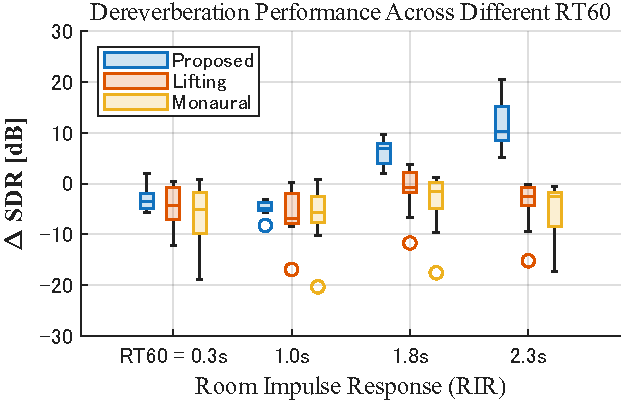
\includegraphics[width=1.0\linewidth]{../Rk1NullspaceOfSylvester_STFTdomain/result/main20260620all.pdf}
\end{figure}

% [IR 1: RT60 = 0.3s]
%   Proposed  : 7.4561 秒
%   Lifting   : 54.1000 秒
%   WPE       : 0.4588 秒
% [IR 2: RT60 = 1.0s]
%   Proposed  : 7.7531 秒
%   Lifting   : 193.7664 秒
%   WPE       : 0.9346 秒
% [IR 3: RT60 = 1.9s]
%   Proposed  : 9.3386 秒
%   Lifting   : 492.3833 秒
%   WPE       : 4.2931 秒
% [IR 4: RT60 = 2.3s]
%   Proposed  : 10.0580 秒
%   Lifting   : 625.0186 秒
%   WPE       : 5.1205 秒

% \begin{figure}
% \centering
% 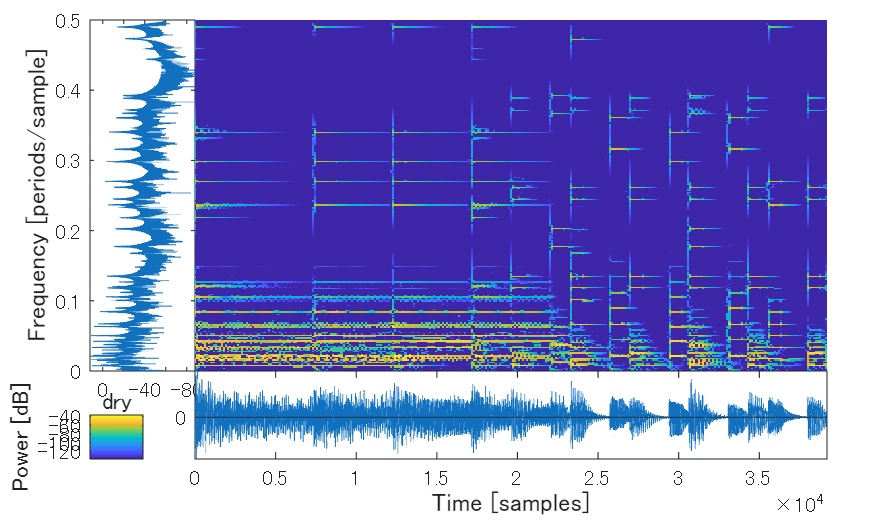
\includegraphics[width=0.8\linewidth]{../Rk1NullspaceOfSylvester_STFTdomain/result/9w3r7y_01_1_dry.png}
% \caption{ドライ音のスペクトログラム}
% 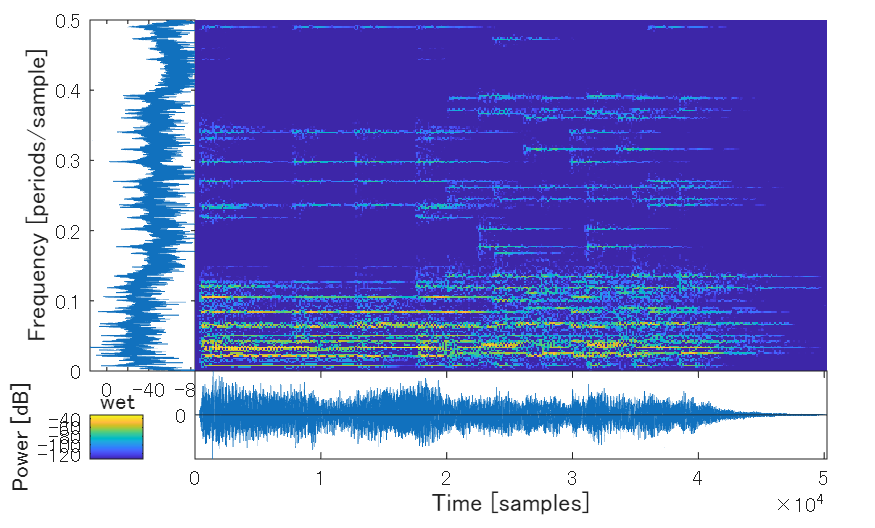
\includegraphics[width=0.8\linewidth]{../Rk1NullspaceOfSylvester_STFTdomain/result/9w3r7y_01_1_wet.png}
% \caption{残響時間$2.6$秒の観測音のスペクトログラム (SDR=$-0.70$ dB)}
% 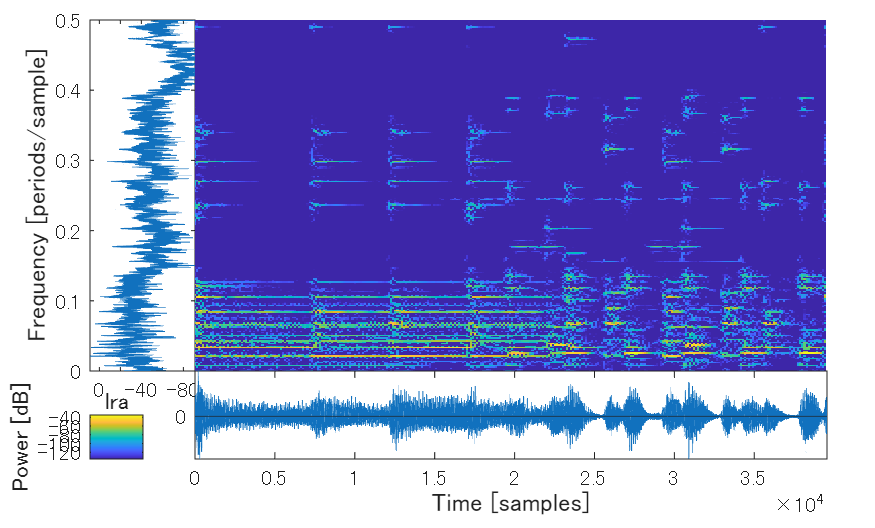
\includegraphics[width=0.8\linewidth]{../Rk1NullspaceOfSylvester_STFTdomain/result/9w3r7y_01_1_ret_pad=-2.png}
% \caption{復元音のスペクトログラム (SDR=$9.06$ dB)}
% \end{figure}

% \begin{figure}
% \centering
% 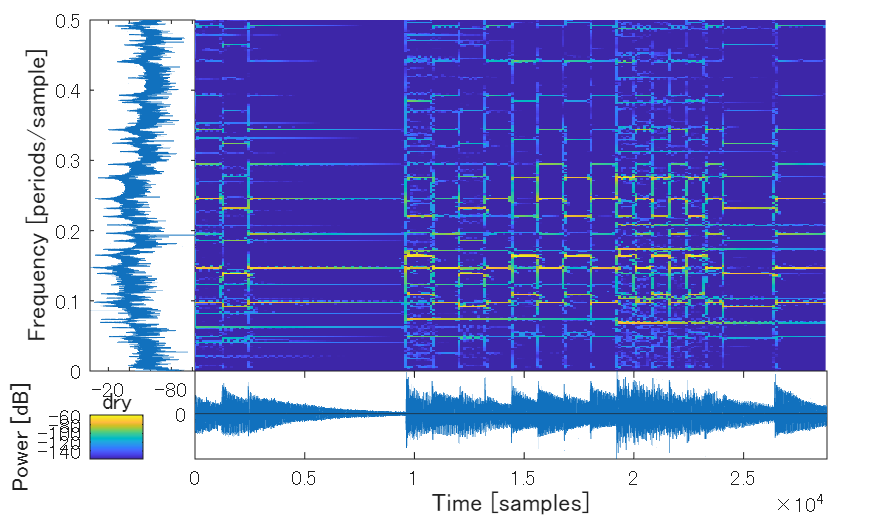
\includegraphics[width=0.8\linewidth]{../Rk1NullspaceOfSylvester_STFTdomain/result/Goldberg_clav_mono_8000_1_dry.png}
% \caption{ドライ音のスペクトログラム}
% 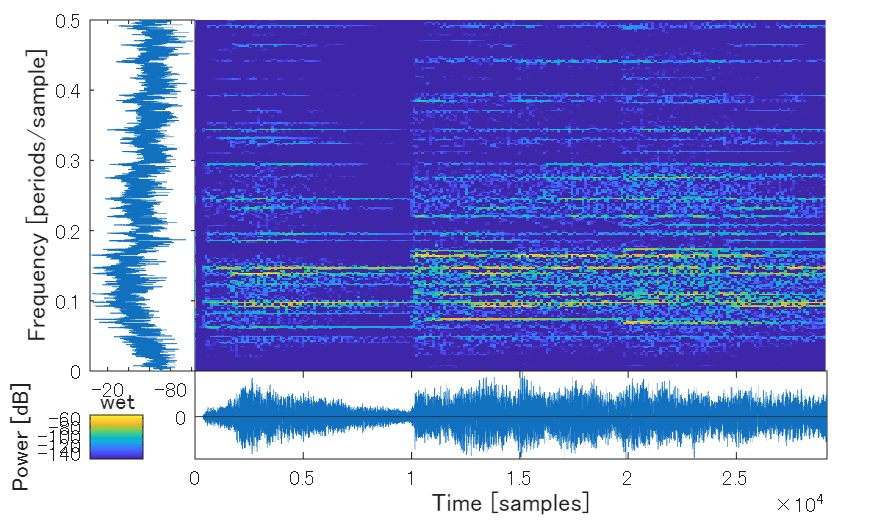
\includegraphics[width=0.8\linewidth]{../Rk1NullspaceOfSylvester_STFTdomain/result/Goldberg_clav_mono_8000_1_wet.png}
% \caption{残響時間$2.6$秒の観測音のスペクトログラム (SDR=$-2.08$ dB)}
% 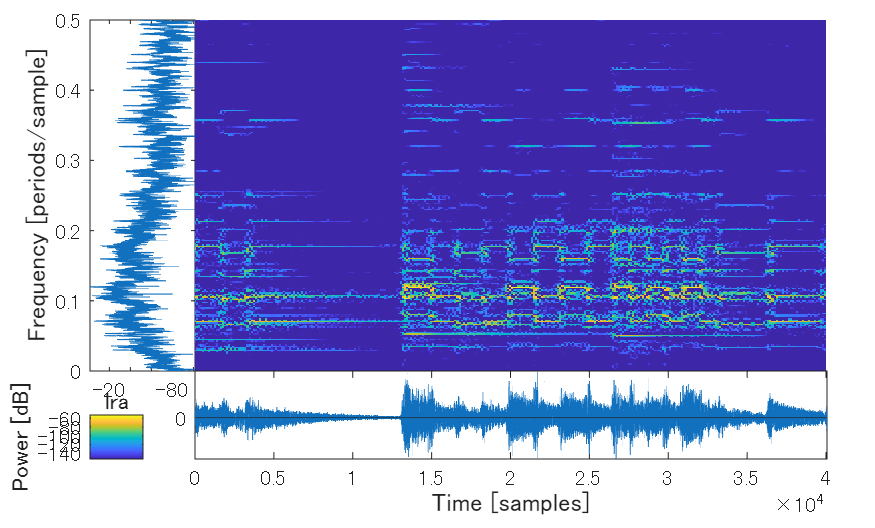
\includegraphics[width=0.8\linewidth]{../Rk1NullspaceOfSylvester_STFTdomain/result/Goldberg_clav_mono_ds_1_ret_pad=-2.png}
% \caption{復元音のスペクトログラム (SDR=$7.17$ dB)}
% \end{figure}

\section{結論}
単チャネル設定におけるブラインド残響除去のための新しい手法を提案した．時間周波数領域でのサブバンド畳み込みモデルに基づく定式化により，長大残響環境下での空間計算量問題を解決しつつ，信号波形の過剰な抑制を回避した．

\footnotesize{
\begin{thebibliography}{1}
  \bibitem{li2018ctf} X. Li, S. Gannot, L. Girin and R. Horaud, "Multichannel Identification and Nonnegative Equalization for Dereverberation and Noise Reduction Based on Convolutive Transfer Function," in IEEE/ACM TASLP, \textbf{26}(10) pp.1755-1768, Oct. 2018,
\end{thebibliography}
}
\end{document}